\chapter{前言}
\renewcommand{\baselinestretch}{10.0} %設定行距
\pagenumbering{arabic} %設定頁號阿拉伯數字
\setcounter{page}{1}  %設定頁數
\fontsize{14pt}{2.5pt}\sectionef
\section{設計架構}
此次專題運用到三大類主題,利用 Solidworks 繪製球場,在 CoppeliaSim 中以虛擬環境創建、模擬和分析複雜的機器人系統, 以 Lua 程式編寫對機器人的操控、設計遊玩規則。\\

\begin{figure}[hbt!]
\begin{center}
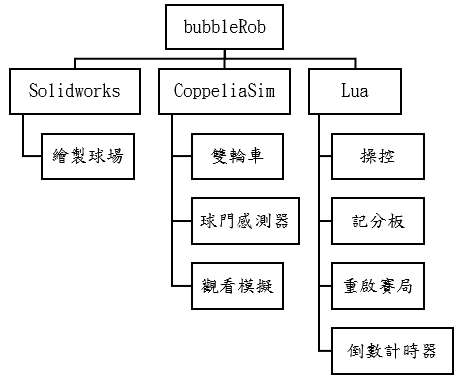
\includegraphics[width=10cm]{ag6設計架構}
\caption{\Large 設計架構圖}\label{fig.ag6設計架構}
\end{center}
\end{figure}

\section{規則說明}
類似於足球遊戲,一開始時球會置於場中央,遊戲開始後兩方即可以鍵盤操控機器人推球至已方的球門得分。\\
遊戲規則如下:
\begin{enumerate}
\item 球觸碰到情們感測器即算得分。
\item 最快獲得5分的隊伍即獲勝。
\item 任一方進球得分後,遊戲會重置,雙方回到場中央重新開球。
\end{enumerate}

\renewcommand{\baselinestretch}{0.5} %設定行距